\subsection{Login and Registration screens}\label{subsec:login-screen}
\textbf{Login screen} (Figure \ref{fig:login_screen}) contains buttons for log in and sign up to the system.
Login buttons allows to log in via email, Google account and it going to add log in via Apple account.
Sign up button allows to sign in only via email.

\textbf{Log in Screen} (Figure \ref{fig:login_screen_log_in}) consists of two text fields.
The first is for typing an e-mail and the other is for typing a password.
After success log in, the user is redirected to \textbf{Dashboard screen}.

\textbf{Sign up screen} (Figure \ref{fig:login_screen_sign_up}) is consist of following three text fields:
\begin{itemize}
    \item the first is for typing an e-mail address through the user will log in to the system,
    \item the second is for typing a password and
    \item the last one is for typing a user name.
\end{itemize}
The last one is optional.
The user has to agree with terms of using before he finishes the registration.
After successful signing up, the user is logged in and redirected to \textbf{Dashboard screen}.


\begin{figure}
    \centering
    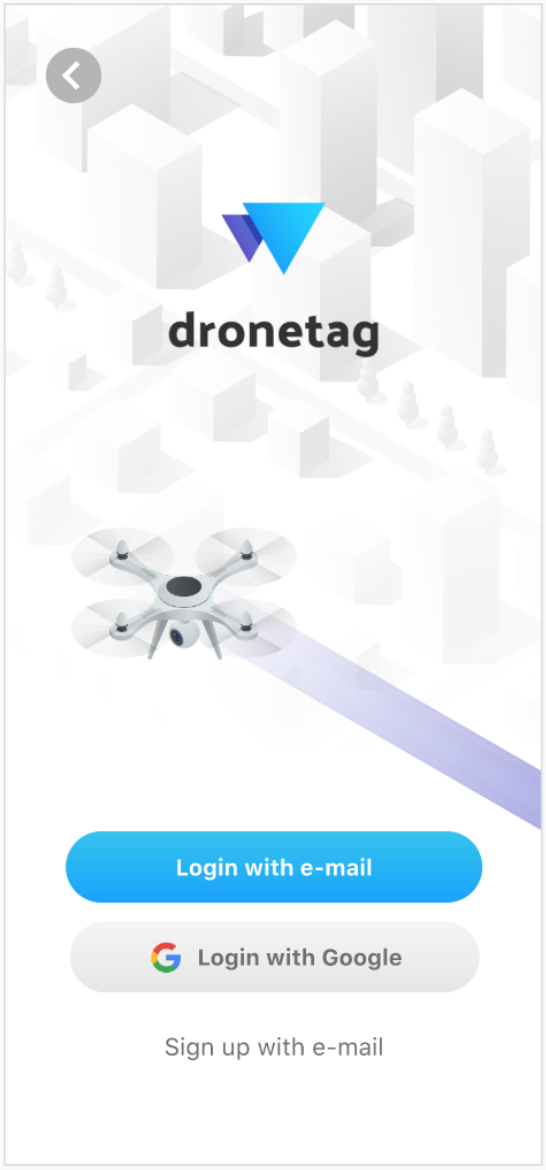
\includegraphics[width=.3\linewidth]{assets/user_interface_design/login/login_screen.png}
    \caption{[A10] Login screen}
    \label{fig:login_screen}
\end{figure}

\begin{figure}
    \centering
    \begin{minipage}{.45\textwidth}
        \centering
        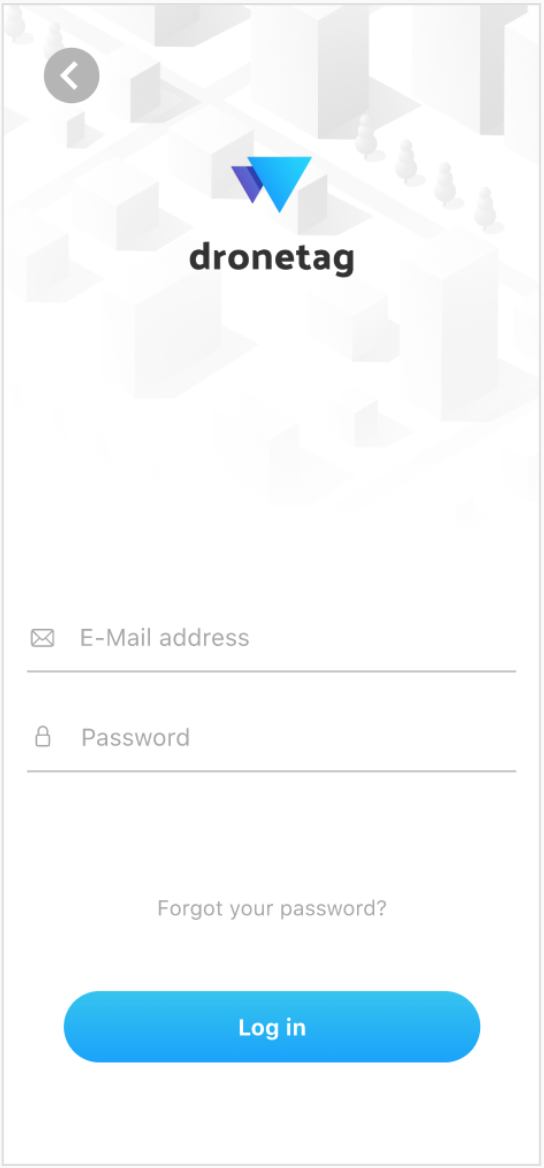
\includegraphics[width=.7\linewidth]{assets/user_interface_design/login/login_screen_log_in.png}
        \caption{[A11] Login screen, log in}
        \label{fig:login_screen_log_in}
    \end{minipage}%
    \hspace{.05\linewidth}
    \begin{minipage}{.45\textwidth}
        \centering
        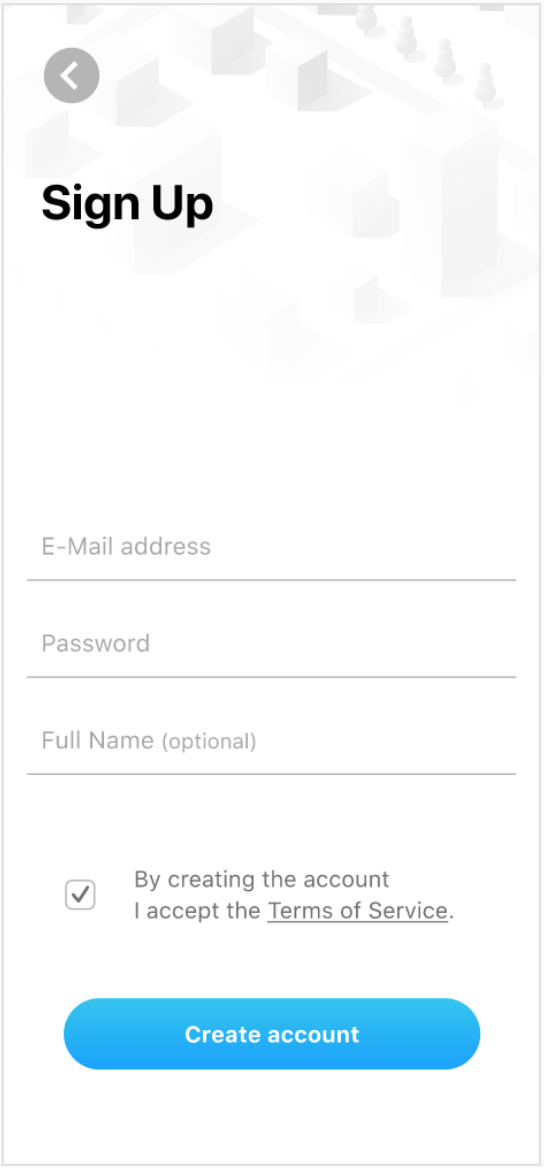
\includegraphics[width=.7\linewidth]{assets/user_interface_design/login/login_screen_sign_up.png}
        \caption{[A12] Login screen, sign up}
        \label{fig:login_screen_sign_up}
    \end{minipage}
    \label{fig:login_screen_all}
\end{figure}
